\section{Swap}
In this section we will describe a set of transformation rules know as swaps. There are two distinct cases of swaps, one in which we swap out a module in a line with a free module that is able to perform the same work as the one it is replacing is currently doing. And one in which we swap out a module within a line, and another module within a line that are capable of the same work as the other is currently doing. These transformations can be beneficial if we swap a faster module with a slower module at a choke point, allowing for more through put.

\subsection{$Swap_0$: External Swap}
For the case of swapping a module out from a configuration with a free module, we have described to transformation rule $Swap_0$, which can be seen in \cref{fig:swap0}.

\begin{figure}[H]
	\centering
	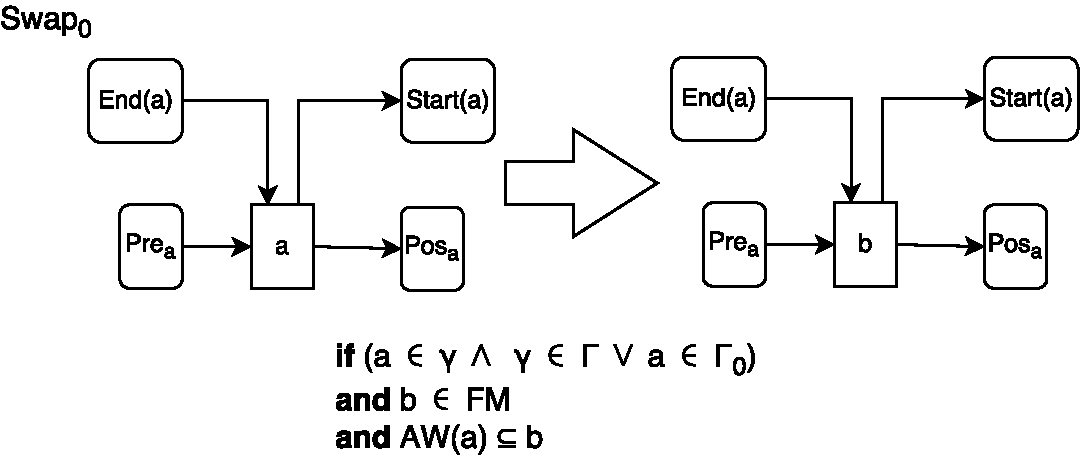
\includegraphics[width=0.7\textwidth]{swap0.pdf}
	\caption{A visual representation of the $Swap_0$ transformation rule}
	\label{fig:swap0}
\end{figure}

Not shown in \cref{fig:swap0} is that we also update the function $AW$ of our new configuration to $AW'$. We define $AW'$ as:

\[AW' = (AW \cup \{(b, AW(a))\} \setminus \{(a, AW(a))\}\]



%We expand our visual representation of our rules with an \texttt{update} clause. This \texttt{update} clause contains a number of update statements, either $add$ and $remove$. The $add$ operation adds a given ordered pair to the function, and the $remove$ operation removes a given ordered pair from the function. An example could be for the function $Foo: X \rightarrow X$ we wish to either add or remove the element $(a, b)$ where $a, b \in X$ then:

%\[Foo.add((a, b)) = Foo \cup \{(a,b)\}\]
%\[Foo.remove((a, b)) = Foo \setminus \{(a,b)\}\]


\subsection{$Swap_1$: Internal Swap}
For the case of swapping a module from a configuration with another module in the same configuration, we have described the transformation rule $Swap_1$, which can be seen in \cref{fig:swap1}.

\begin{figure}[H]
	\centering
	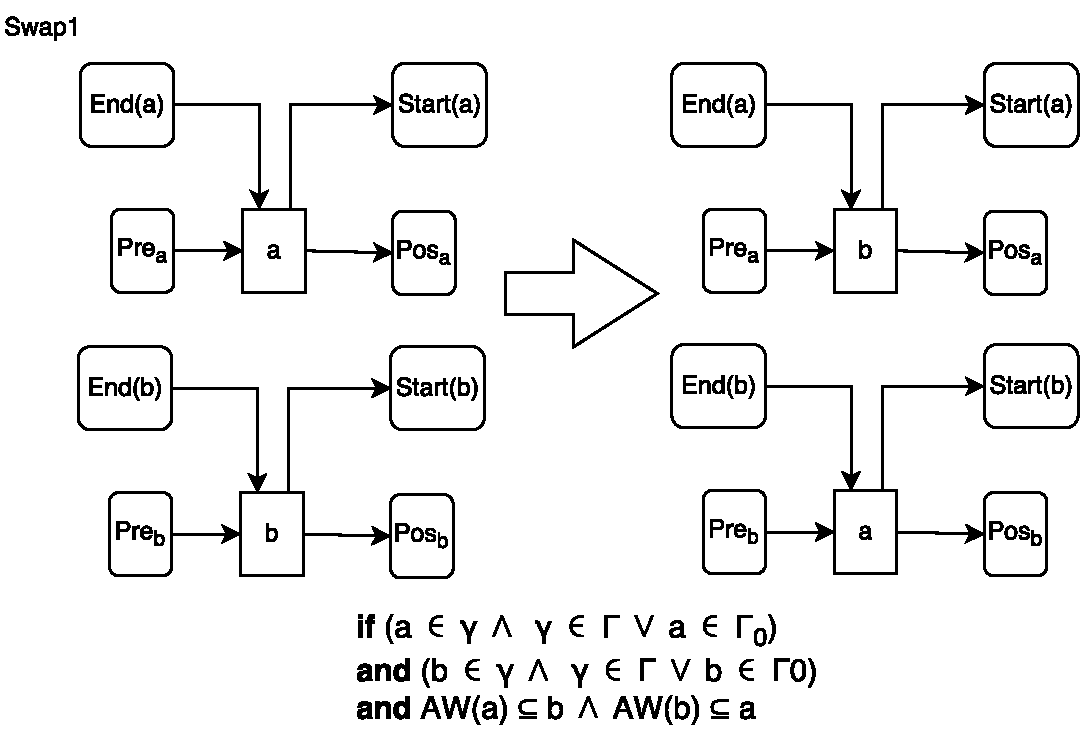
\includegraphics[width=0.7\textwidth]{swap1.pdf}
	\caption{A visual representation of the $Swap_1$ transformation rule}
	\label{fig:swap1}
\end{figure}

Not shown in \cref{fig:swap1} is that we also update the function $AW$ of our new configuration to $AW'$. We define $AW'$ as:

\[AW' = (AW \cup \{(b, AW(a)), (a, AW(b)\} \setminus \{(a, AW(a)), (b, AW(b))\}\]


